\appendix

% Agent任务的 LLM 时间占比与瓶颈
\section{LLM Time Breakdown and Bottleneck Analysis in Agent Tasks}
\label{llm-time-ratio}

\begin{table}[H]
    \vspace{-10pt}
    \centering
    \caption{LLM inference time breakdown across agent tasks.}
    \label{tab:llm_time_breakdown}
    \begin{tabular}{llccc}
        \toprule
        \textbf{Task} & \textbf{Dataset} & \textbf{Avg. JCT (s)} & \textbf{Avg. LLM Time (s)} & \textbf{LLM Time Ratio} \\
        \midrule
        Web Search & 2WikiMultihopQA & 60.36 & 36.49 & 60.46\% \\
        Web Search & Bamboogle       & 49.15 & 32.91 & 66.95\% \\
        Web Search & HotpotQA        & 40.72 & 29.14 & 71.56\% \\
        Coding     & MBPP            & 30.10 & 30.06 & 99.87\% \\
        \bottomrule
    \end{tabular}
\end{table}

\begin{figure}[!b]
    \begin{center}
    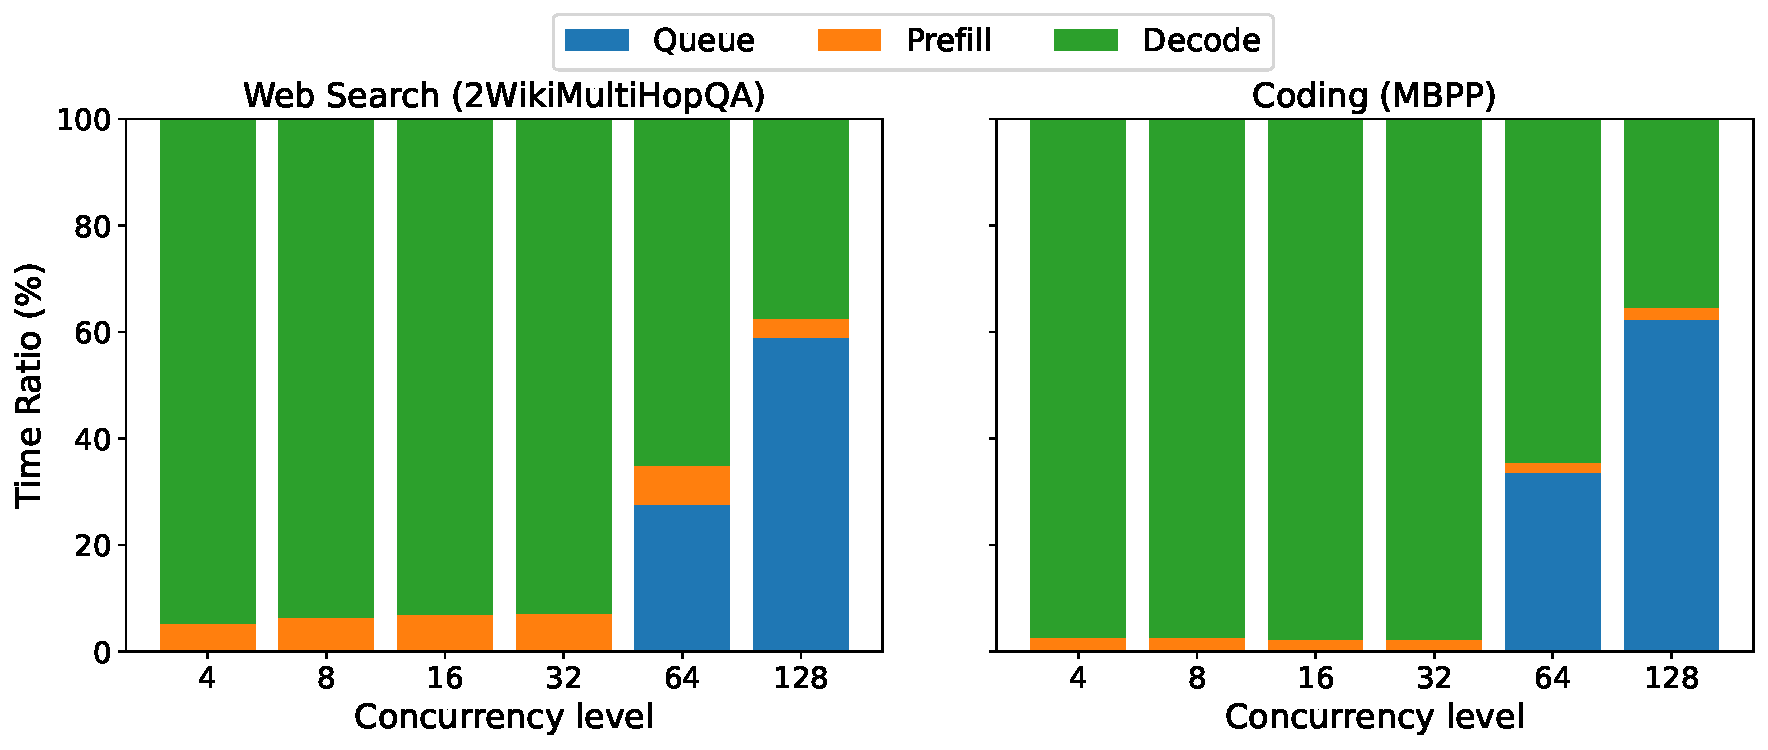
\includegraphics[width=1.0\linewidth]{figures/5-time-ratio.pdf}
    \end{center}
    \caption{
        LLM inference time breakdown under different concurrency levels for two agent tasks, Web Search on 2WikiMultihopQA and Coding on MBPP, showing a shift from decode-dominated latency at low concurrency to queue-dominated latency at high concurrency.
    }
    \label{fig:llm_time_ratio}
\end{figure}

We measure the end-to-end execution time and the fraction spent on LLM inference across different agent tasks and datasets, as shown in~\autoref{tab:llm_time_breakdown}.
LLM inference accounts for the majority of the end-to-end latency across all evaluated settings.
For some tasks, the execution time of external tools is negligible, making LLM inference responsible for nearly all of the overall latency.
These results indicate that the end-to-end latency of agent tasks is primarily bottlenecked by LLM inference.
Coding and Web Search tasks typically represent two contrasting cases.
In Coding tasks, the tool execution mainly consists of running generated code and is usually very fast, whereas in Web Search tasks, the agent often needs to retrieve and access multiple webpages, making tool execution more sensitive to network latency.
Despite this difference, LLM inference still accounts for a substantial fraction of the end-to-end latency in both types of tasks.

We further analyze the latency breakdown of LLM requests in agent tasks, as shown in~\autoref{fig:llm_time_ratio}.
The latency of an LLM request mainly consists of three components: prefill, decode, and queueing time.
Existing serving systems have extensively optimized KV-cache reuse, substantially reducing redundant computation during the prefill stage and making prefill latency relatively small.
To preserve KV-cache residency and avoid excessive eviction or recomputation, these systems typically employ admission control based on the number of concurrent requests and the available KV-cache capacity.
When the number of concurrent requests exceeds the capacity that can be supported by the available KV cache, newly arrived requests are queued and can enter inference only after running requests complete and release their KV-cache space.

Based on these results, we observe a concurrency-dependent shift in the LLM inference bottleneck of agent tasks.
At low concurrency, decode time dominates the request latency and serves as the primary performance bottleneck.
As concurrency increases, more requests are blocked by admission control, causing queueing time to grow rapidly and eventually dominate the overall latency.
As a result, the performance bottleneck shifts from decoding at low serving loads to queueing at high serving loads.

\clearpage

% Agent任务使用 SD 的加速比随 Batch Size 的变化关系
\section{Impact of Batch Size on SD Speedup for Agent Tasks}
\label{sd-speedup}

% 暂时占个位置
\clearpage

% 对比不同动态 SD 方法
\section{Comparison of Dynamic SD Approaches.}
\label{dynamic-sd-comparison}

\begin{table}[H]
    \vspace{-20pt}
    \centering
    \caption{Token consistency comparison across different approaches of dynamic SD.}
    \label{tab:token_consistency}
    \begin{tabular}{cccc}
        \toprule
        \textbf{Inference Engine} & \textbf{Engine A} & \textbf{Engine B} & \textbf{Token Consistency} \\
        \midrule

        \multirow{4}{*}{vLLM}
        & Dynamic SD ($\text{draft\_len}=0$)
        & NonSD
        & $\times$ \\

        & Dynamic SD ($\text{draft\_len}=0$)
        & SD
        & $\checkmark$ \\

        & SpecSys-NonSD Mode
        & NonSD
        & $\checkmark$ \\

        & SpecSys-SD Mode
        & SD
        & $\checkmark$ \\

        \midrule

        \multirow{4}{*}{SGLang}
        & Adaptive SD ($\text{draft\_len}=0$)
        & NonSD
        & $\times$ \\

        & Adaptive SD ($\text{draft\_len}=0$)
        & SD
        & $\checkmark$ \\

        & SpecSys-NonSD Mode
        & NonSD
        & $\checkmark$ \\

        & SpecSys-SD Mode
        & SD
        & $\checkmark$ \\

        \bottomrule
    \end{tabular}
\end{table}

\textbf{Token Consistency across Dynamic SD Approaches.}
Online inference engines typically employ different execution paths for SD and Non-SD generation to improve efficiency, with different kernels used for key computations such as attention.
As a result, even under deterministic decoding settings (i.e., temperature $=0$ and top-$k=1$), SD and Non-SD execution may generate slightly different token sequences for the same prompt due to differences in their underlying computation paths, although the generated contents are usually semantically similar.
Therefore, token-level consistency provides a practical indicator of whether two execution modes follow the same underlying inference path.
We evaluate this behavior for two dynamic SD approaches, vLLM Dynamic SD and SGLang Adaptive SD, as shown in~\autoref{tab:token_consistency}.
For both vLLM Dynamic SD and SGLang Adaptive SD, when SD is disabled by setting $\text{draft\_len}=0$, the generated tokens are inconsistent with those of the native Non-SD engine but remain consistent with those produced by the native SD engine.
This indicates that setting $\text{draft\_len}=0$ does not fully switch execution back to the native Non-SD path; instead, the engine continues to follow the SD execution path with SD disabled.
In contrast, SpecSys's Non-SD mode produces tokens consistent with the native Non-SD engine, while its SD mode remains consistent with the native SD engine.
These results demonstrate that SpecSys performs a more complete runtime switch between the native SD and Non-SD execution paths.

\textbf{Non-SD Overhead across Dynamic SD Approaches.}
Since vLLM Dynamic SD and SGLang Adaptive SD continue to execute along the SD path when $\text{draft\_len}=0$, this path is suboptimal for autoregressive Non-SD generation and introduces additional performance overhead.
We therefore measure the Non-SD execution overhead of these two dynamic SD approaches and SpecSys relative to the native Non-SD engine, as shown in~\autoref{fig:nonsd_overhead}.
However, SpecSys consistently incurs substantially lower overhead than vLLM Dynamic SD and SGLang Adaptive SD across all batch sizes.
These results further demonstrate the benefit of SpecSys's more complete runtime switching between the native SD and Non-SD execution paths.

\begin{figure}[!b]
    \begin{center}
    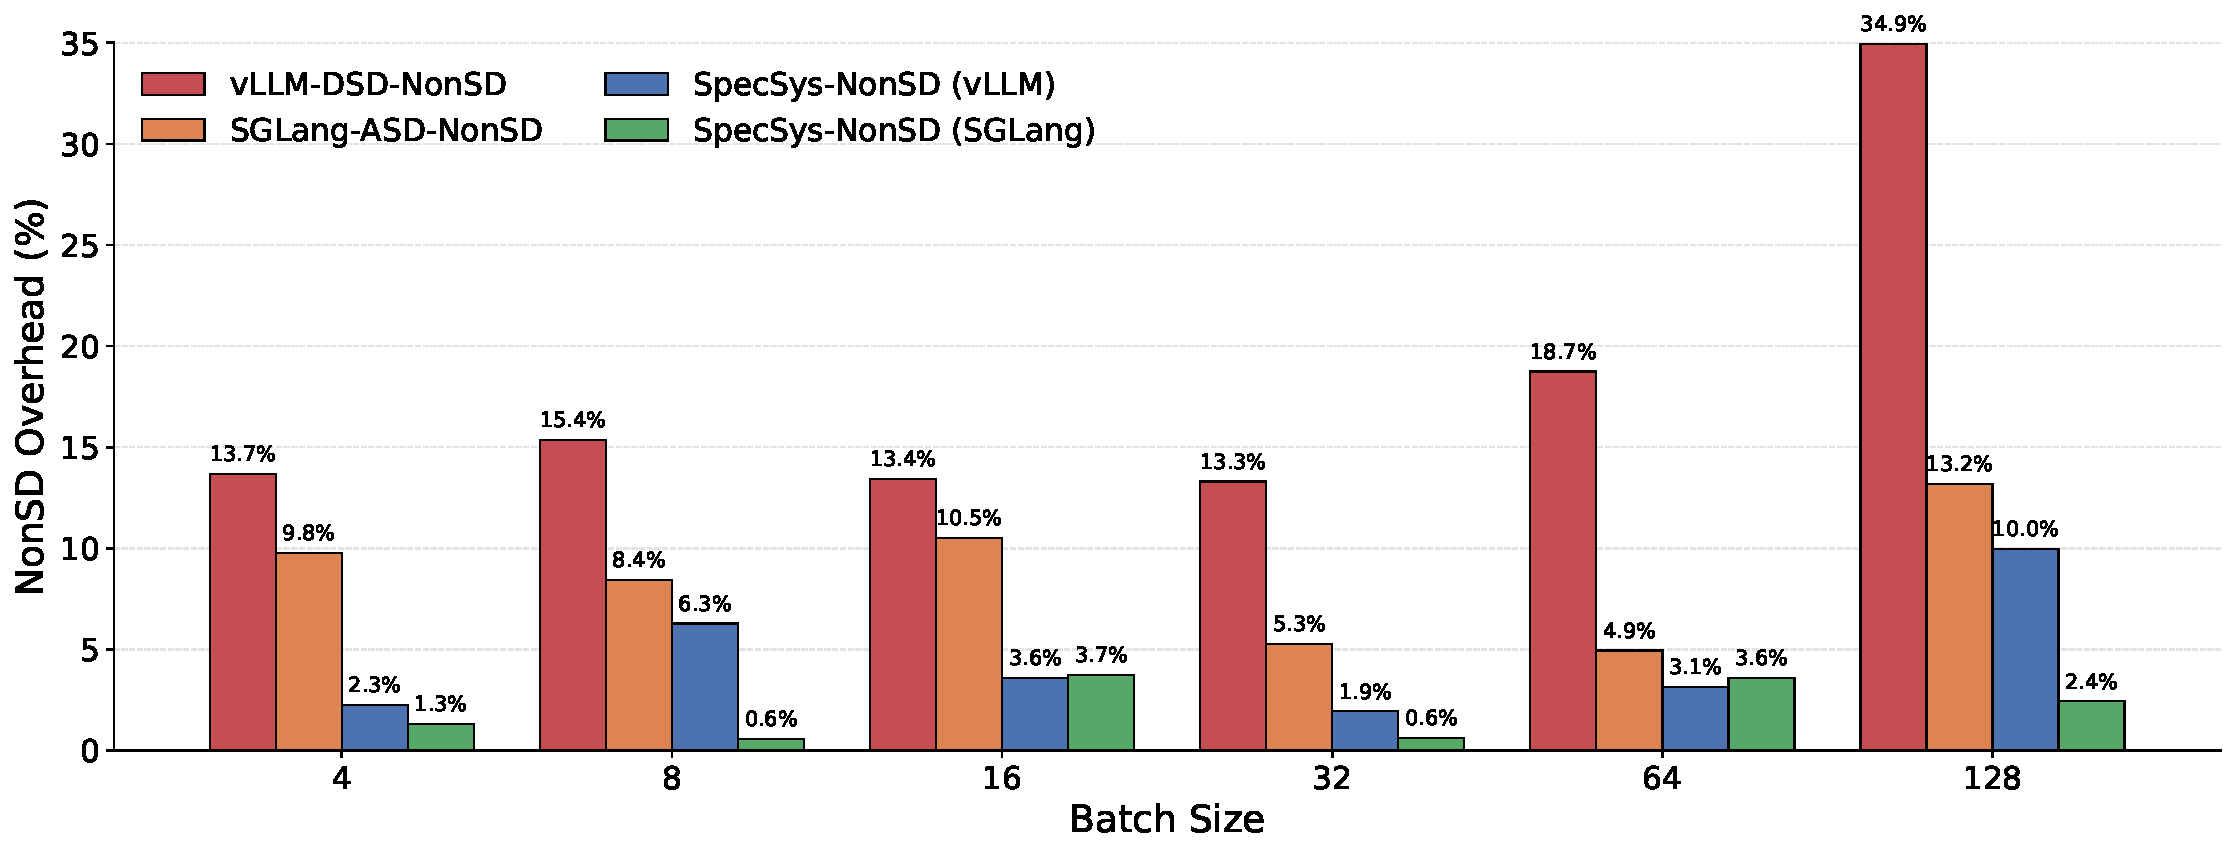
\includegraphics[width=1.0\linewidth]{figures/6-nonsd-overhead.pdf}
    \end{center}
    \caption{
        Non-SD execution overhead across different dynamic SD approaches and batch sizes.
    }
    \label{fig:nonsd_overhead}
\end{figure}


% 列举不同 workflow 和 workload 的 step 分布
\section{Agent Step Distributions across Workflows and Workloads}
\label{step-distribution}

% 暂时占个位置
\clearpage

% prompt 解析的实例
\section{Examples of Prompt Parsing}
\label{prompt_parser}

% 暂时占个位置
\clearpage

% 轨迹的请求变化图
\section{Request Arrival Patterns of Online Serving Traces}
\label{online-trace-detail}

\begin{figure}[H]
    \begin{center}
    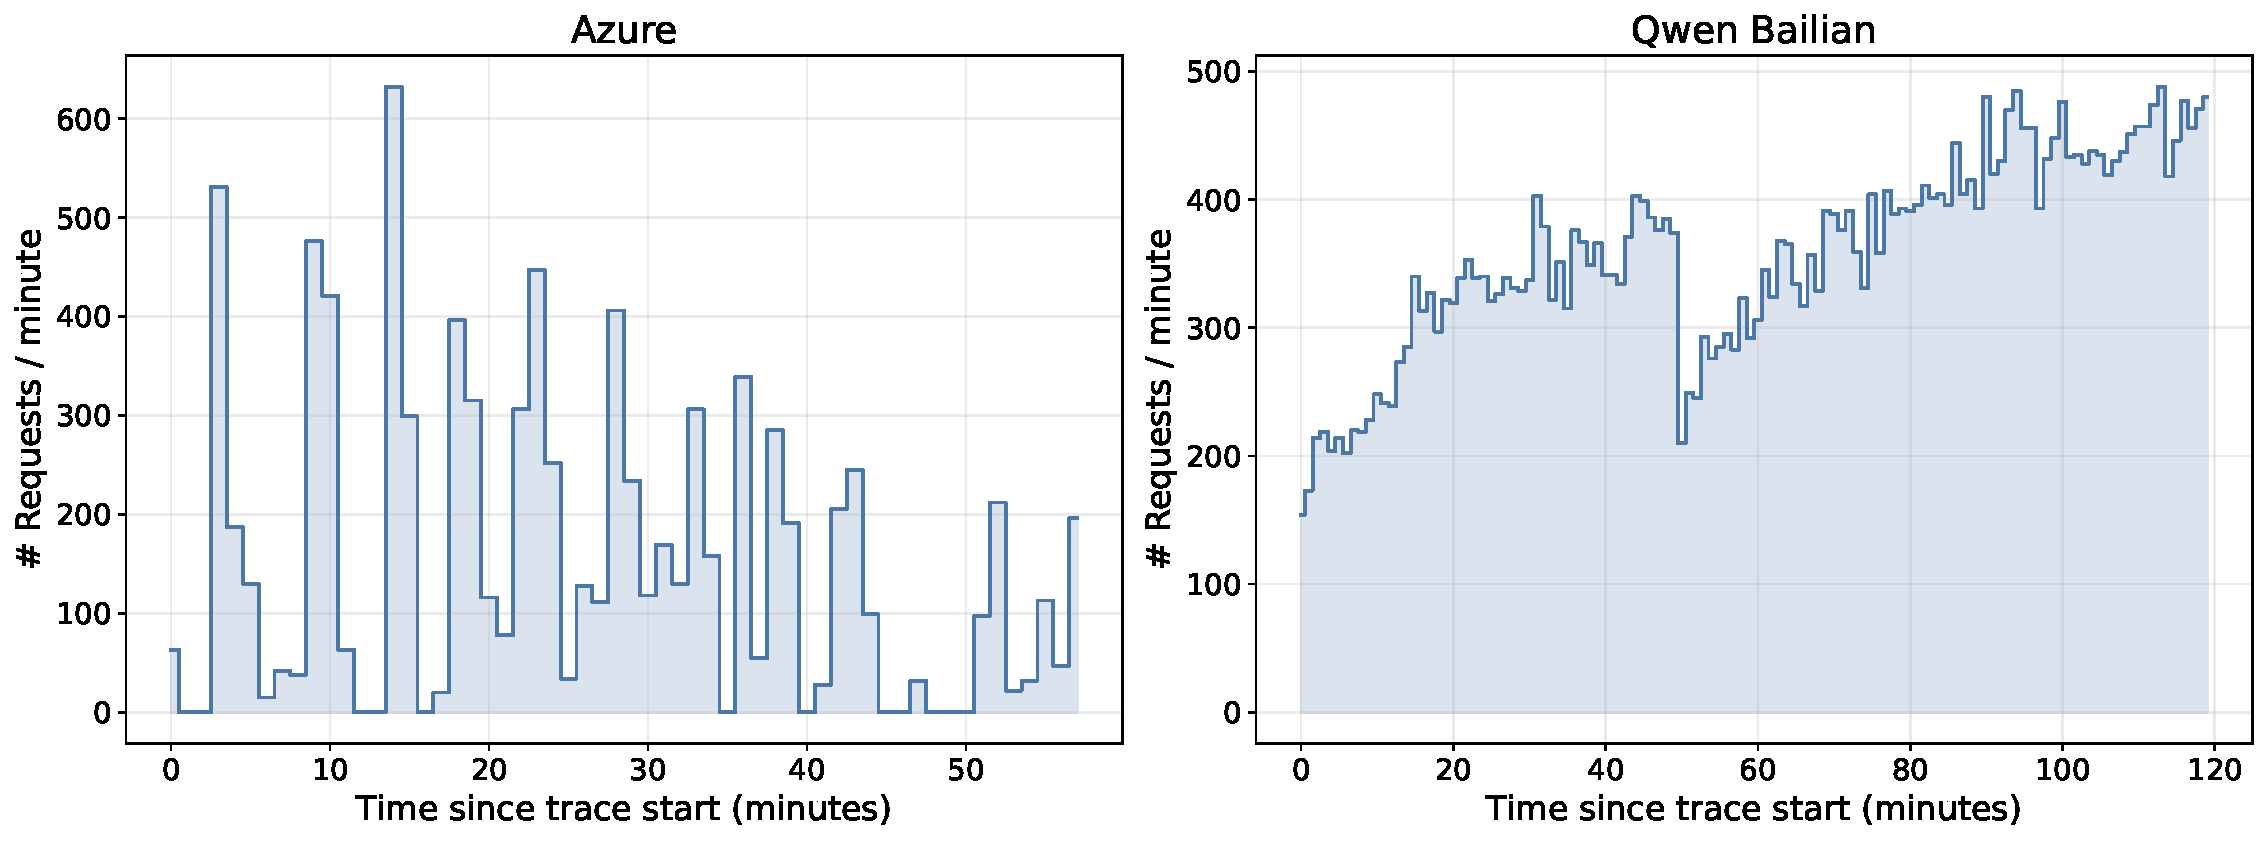
\includegraphics[width=1.0\linewidth]{figures/online-request-trace.pdf}
    \end{center}
    \caption{
        Request arrival patterns of the Azure and Qwen Bailian traces, measured as the number of requests per minute over time.
    }
    \label{fig:online_request_trace}
\end{figure}

We further examine the request-volume dynamics of the two online inference traces used in our end-to-end evaluation, as shown in Figure~\ref{fig:online_request_trace}, and summarize their key statistics in Table~\ref{tab:trace_statistics}.

\textbf{Azure Trace.}
The Azure trace exhibits highly bursty traffic, with frequent alternations between low-load periods and sharp traffic spikes.
Its average arrival rate is 152.05 requests/min, while the peak reaches 632 requests/min, about 4.16$\times$ the average.
Such rapid load fluctuations make SD beneficial during low-load periods, but may cause performance degradation when sudden bursts push the serving system into a high-load regime.
Therefore, this trace is well suited for evaluating whether dynamic SD methods can effectively adapt their SD decisions to rapidly changing serving loads.

\textbf{Qwen Bailian Trace.}
In contrast, the Qwen Bailian trace is considerably smoother and remains under sustained high load for most of its duration.
Its average arrival rate reaches 358.82 requests/min, more than twice the 152.05 requests/min observed in the Azure trace, while its peak is 488 requests/min.
Under such consistently high load, the benefit of SD is limited and can even cause performance degradation, while a large number of requests may accumulate in the waiting queue.
This trace is therefore well suited for evaluating both the Non-SD overhead introduced by dynamic SD mechanisms under high load and the effectiveness of task scheduling strategies in reducing queueing delay.

\begin{table}[H]
    \centering
    \caption{Statistics of the Azure and Qwen Bailian traces.}
    \label{tab:trace_statistics}
    \begin{tabular}{lrrrrr}
        \toprule
        \textbf{Trace} &
        \textbf{\# Requests} &
        \textbf{Duration (min)} &
        \textbf{Avg. Req./min} &
        \textbf{Peak Min.} &
        \textbf{Peak Req.} \\
        \midrule
        Azure         & 8,819  & 57.27  & 152.05 & 14  & 632 \\
        Qwen Bailian  & 43,058 & 119.99 & 358.82 & 113 & 488 \\
        \bottomrule
    \end{tabular}
\end{table}


\clearpage

% 不同硬件平台的资源分析
\section{Serving Capacity Analysis}
\label{resource-analysis}

% 暂时占个位置
\clearpage

% 不同通信频率的影响
\section{Impact of Communication Frequency on System Performance}
\label{communication-frequency}

% 暂时占个位置
\clearpage

% 预测-调度策略的额外开销
\section{Overhead of SpecSys Prediction and Scheduling}
\label{prediction-scheduling-overhead}

% 暂时占个位置
\clearpage